% last updated in April 2002 by Antje Endemann
% Based on CVPR 07 and LNCS, with modifications by DAF, AZ and elle, 2008 and AA, 2010, and CC, 2011; TT, 2014; AAS, 2016

\documentclass[runningheads]{llncs}
\usepackage{graphicx}
\usepackage{amsmath,amssymb} % define this before the line numbering.
\usepackage{ruler}
\usepackage{color}
\usepackage[width=122mm,left=12mm,paperwidth=146mm,height=193mm,top=12mm,paperheight=217mm]{geometry}
\begin{document}
% \renewcommand\thelinenumber{\color[rgb]{0.2,0.5,0.8}\normalfont\sffamily\scriptsize\arabic{linenumber}\color[rgb]{0,0,0}}
% \renewcommand\makeLineNumber {\hss\thelinenumber\ \hspace{6mm} \rlap{\hskip\textwidth\ \hspace{6.5mm}\thelinenumber}}
% \linenumbers
\pagestyle{headings}
\mainmatter
\def\ECCV18SubNumber{27}  % Insert your submission number here

\title{Directional Pseudo-color Enhancement of Image Gradients} % Replace with your title

\titlerunning{ECCV-18 submission ID \ECCV18SubNumber}

\authorrunning{ECCV-18 submission ID \ECCV18SubNumber}

\author{Anonymous ECCV submission}
\institute{Paper ID \ECCV18SubNumber}


\maketitle

\begin{abstract}
Computing an image gradient is a common image filtering task in computer vision and is used to quantify the magnitude and direction of the edges in an image. Whether used to detect edges or to serve as features for downstream classification tasks, the image gradient highlights salient features in an image. Typically, the image gradient is represented as a grayscale image. This paper presents an approach to color the edges of an image (the image gradient) in a deliberate, coherent, and artistic manner. By using the direction of the image gradient to pseudo-color the magnitude of the image gradient, we can enhance the visual quality of the gradient. The result is an image that resembles a skeleton of the original image, colored consistently according to edge direction, and contrasted against a black background.
\keywords{image filtering, edge detection, pseudo-coloring}
\end{abstract}

\section{Introduction}

Edge detection is a fundamental image processing technique that uses an image gradient to quantify the magnitude and direction of the edges in an image. In this paper, we introduce a technique to color the edges of an image in a deliberate, coherent, and artistic manner. An example is shown in Figure 1.

\begin{figure}
\centering
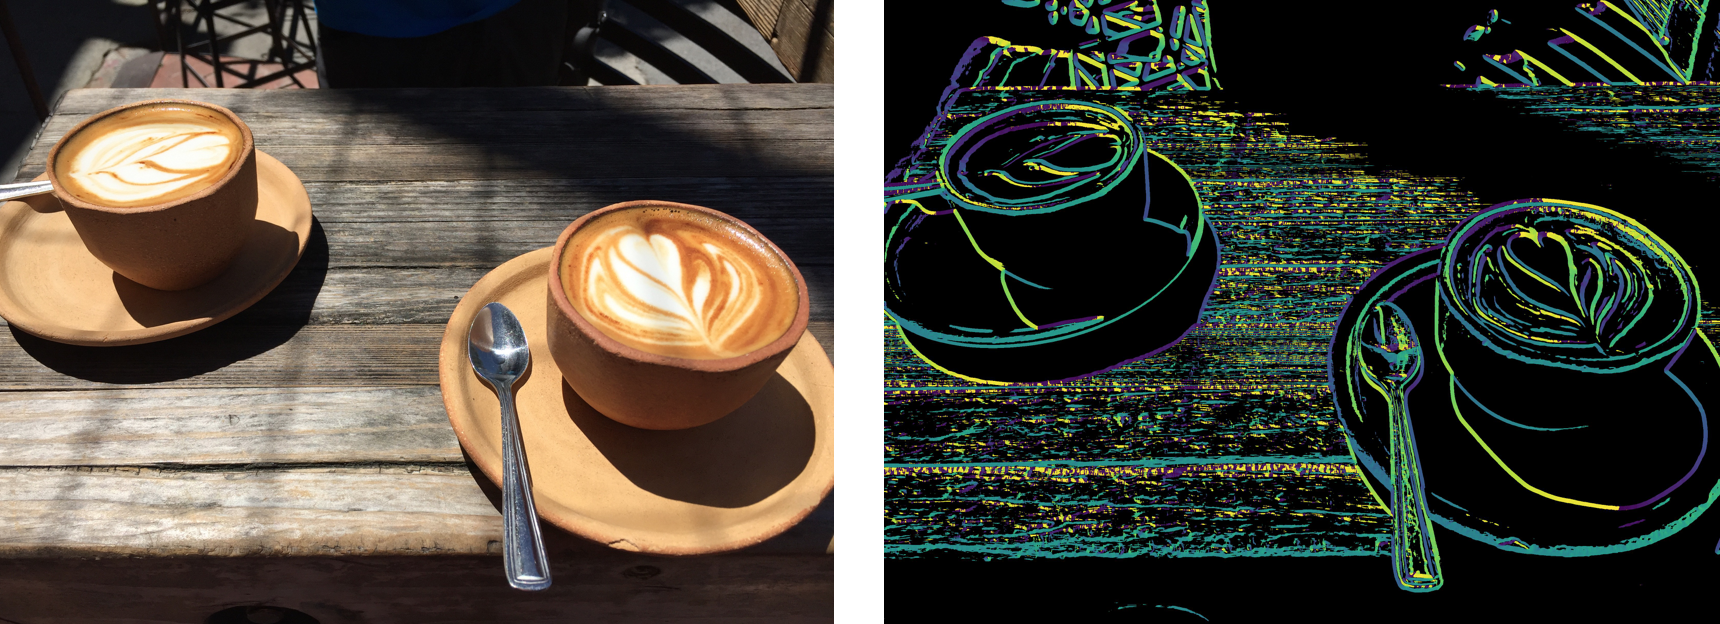
\includegraphics[height=4.4cm]{images/intro.png}
\caption{A demonstration of the approach. Left: The original image. Right: The image gradient magnitude pseudo-colored by the image gradient direction.}
\label{fig:example}
\end{figure}

Image gradients are important because they serve as components for various downstream tasks in computer vision such as edge detection and image classification. However, the image gradients themselves are dull. Image gradients are typically represented as grayscale or black-and-white images depicting the change in intensity at each pixel of the original image, as in the right-hand panel of Figure 2.

\begin{figure}
\centering
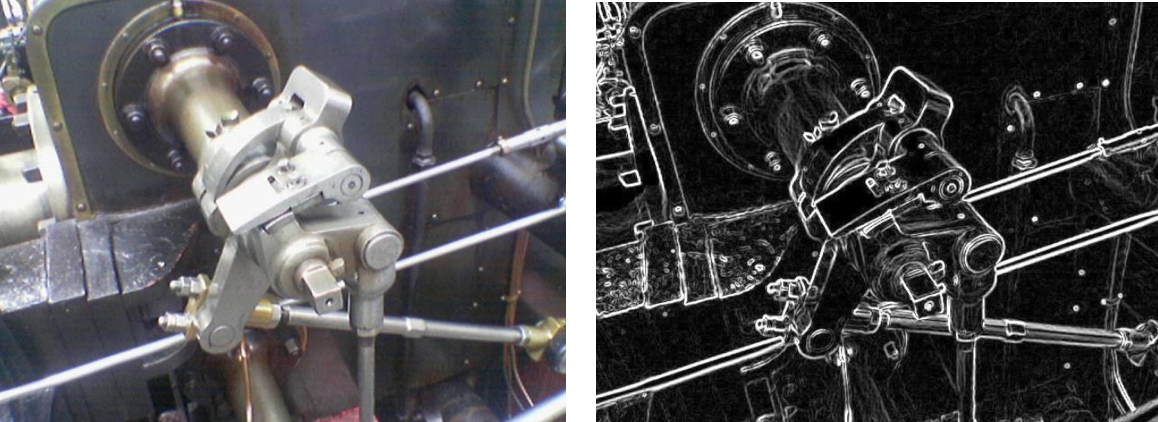
\includegraphics[height=4cm]{images/image_gradient.png}
\caption{The image gradient magnitude (right) is a grayscale image showing the change in intensity at each pixel of the original image (left).}
\label{fig:example}
\end{figure}

The goal of this paper is to make image gradients more appealing and informative by enhancing them with color. The human eye can discern thousands of shades of color, but only two-dozen shades of gray \cite{human_machine}. So, a better, more visible image gradient will reveal details that were not visible in the grayscale gradient. Further, we hope that a colored image gradient will create an artistic representation of the original image that is aesthetically pleasing.

\section{Methodology}

The proposed pipeline for coloring the edges of an image has two main parts: edge detection and edge coloring. We combine a series of convolutions and other linear algebra operations to blur the image, detect its edges, compute gradient magnitude and directions, and pseudo-color the gradient magnitude.

\subsection{Edge detection}

The standard approach for edge detection is to convolve an image with a derivative filter like the Sobel filter to differentiate the intensity of the image pixels with respect to the horizontal and vertical directions of the image. However, since differentiation is very sensitive to noise, it is useful to blur the image first [2]. This can be achieved by convolving the original image $f$ with a blur filter, such as the Gaussian filter, to produce a blurred image $f_b$. For the purposes of edge detection, we will first convert $f$ to a grayscale image. Figure 3 shows the blur transformation.

\begin{align}
f_b = f * \begin{bmatrix} 
1 & \quad 2 & \quad 1 \\ 
2 & \quad 4 & \quad 2 \\ 
1 & \quad 2 & \quad 1  
\end{bmatrix}
\end{align}

\begin{figure}
\centering
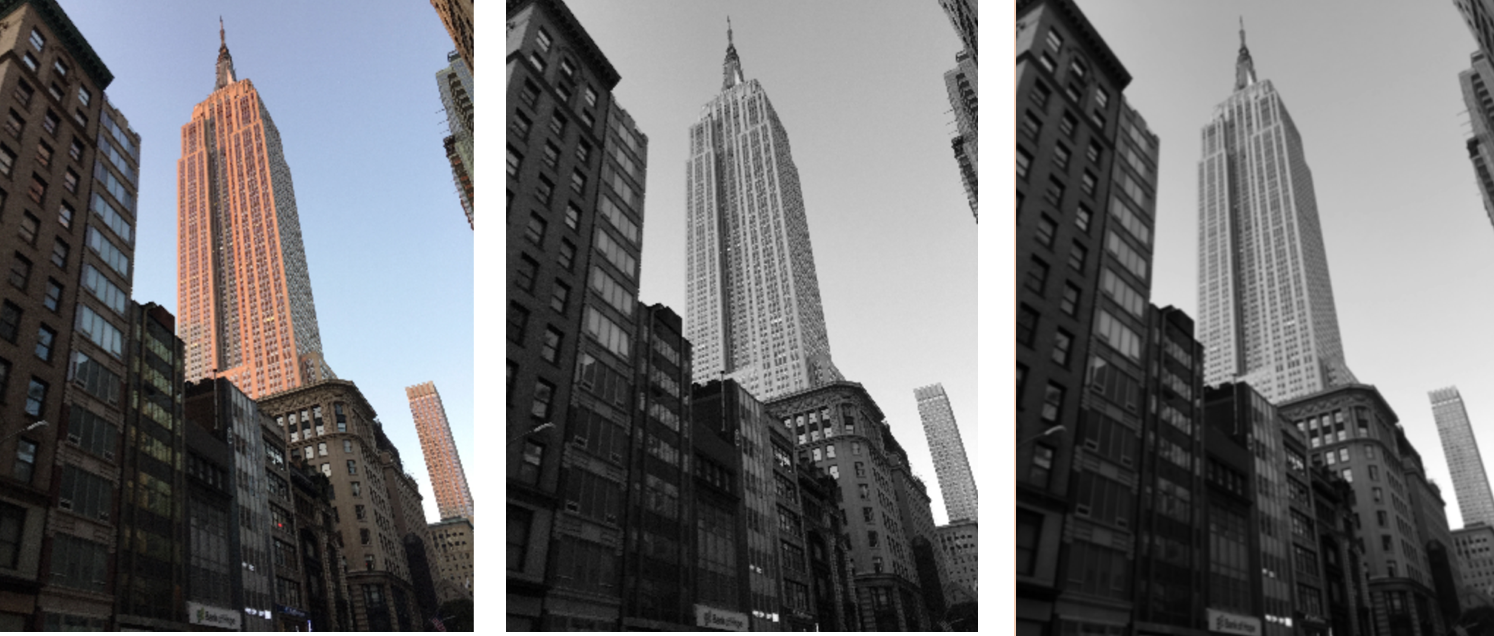
\includegraphics[height=5cm]{images/blur.png}
\caption{Blurring denoises the image and makes it easier to detect edges. The original image (left) is converted to grayscale (middle) and then blurred (right) using a blur filter.}
\label{fig:example}
\end{figure}

Once the image has been blurred, we can perform edge detection using Sobel filters [3]. We convolve the blurred image $f_b$ with the horizontal and vertical Sobel filters, $S_x$ and $S_y$ respectively, to approximate the image derivatives in the horizontal and vertical directions, $\frac{\partial f_b}{\partial x}$ and $\frac{\partial f_b}{\partial y}$ respectively. $\frac{\partial f_b}{\partial x}$ has a strong response for vertical edges, and $\frac{\partial f_b}{\partial y}$ has a strong response for horizontal edges.

\begin{align}
S_x = \begin{bmatrix} 
1 & \quad 0 & \quad -1 \\ 
2 & \quad 0 & \quad -2 \\ 
1 & \quad 0 & \quad -1  
\end{bmatrix}
\quad S_y = \begin{bmatrix} 
1 & \quad 2 & \quad 1 \\ 
0 & \quad 0 & \quad 0 \\ 
-1 & \quad -2 & \quad -1  
\end{bmatrix}
\end{align}

\begin{align}
\frac{\partial f_b}{\partial x} &= f_b * S_x \\
\frac{\partial f_b}{\partial y} &= f_b * S_y
\end{align}

$\frac{\partial f_b}{\partial x}$ and $\frac{\partial f_b}{\partial y}$ can be combined to form the image gradient $\nabla f$. The following equations show how to calculate the magnitude $G$ and the direction $\theta$ of the image gradient. The resulting image gradient magnitude represents the intensity of edges in the image and is shown in Figure 4.

\begin{align}
\nabla f_b &= \begin{bmatrix} \frac{\partial f_b}{\partial x}, \frac{\partial f_b}{\partial y} \end{bmatrix} \\
G &= \vert \vert \nabla f_b \vert \vert = \sqrt{\Big( \frac{\partial f_b}{\partial x} \Big)^2 + \Big( \frac{\partial f_b}{\partial y} \Big)^2} \\
\theta &= tan^{-1} \Big(\frac{\partial f_b}{\partial x} / \frac{\partial f_b}{\partial y})
\end{align}

\begin{figure}
\centering
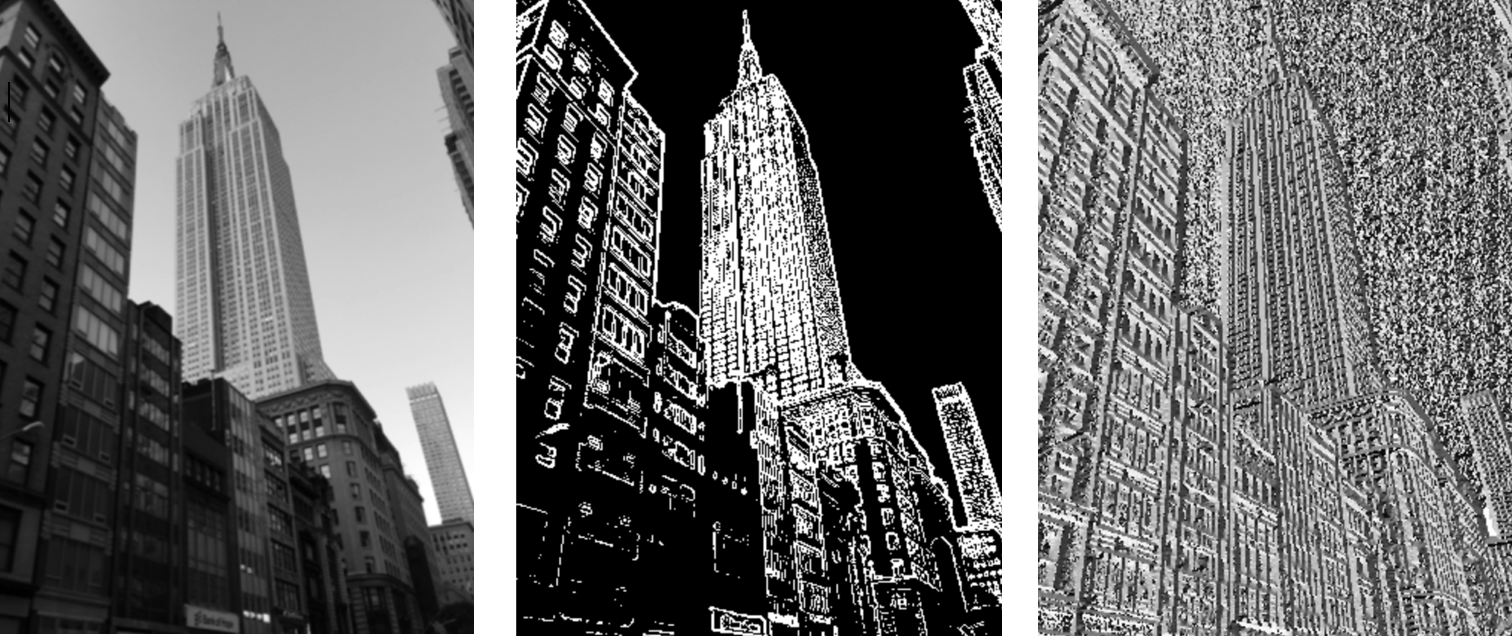
\includegraphics[height=5cm]{images/edge.png}
\caption{Edge detection using Sobel filters. We convolve the blurred image (left) with the Sobel filters and compute the magnitude (middle) and direction (right) of the gradient.}
\label{fig:example}
\end{figure}

Although the gradient magnitude image describes the edges in the original image, it lacks artistic quality and novelty. Next, we consider how to color this gradient magnitude to turn it into a vibrant piece of art.

\subsection{Edge coloring}

\section{Results}

\section{Conclusion}


\bibliographystyle{splncs}
\bibliography{egbib}
\end{document}
